\chapter{Processamento de Linguagem Natural}
\label{cap:Processamento}

% Um computador, obviamente, está preparado para entender sua própria linguagem,
% como por exemplo, um compilador interpreta linhas de código fonte para gerar um
% programa executável seguindo exatamente o algoritmo utilizado. Por isso, temos o
% termo Natural no Processamento de Linguagem.

O objetivo da área de Processamento de Linguagem Natural é analisar a linguagem
natural, ou seja, a linguagem utilizada pelo seres humanos seja ela escrita
ou falada \cite{manningschutze1999}.

O Processamento de Linguagem Natural é uma área antiga, sendo anterior a
invenção dos computadores modernos. De fato, sua primeira grande aplicação foi
um dicionário desenvolvido no Birkbeck College em Londres no ano de 1948. Por ser
uma área complexa, seus primeiros trabalhos foram notavelmente falhos o que
causou uma certa hostilidade por parte das agências fomentadoras de pesquisas.

Os primeiros pesquisadores eram muitas vezes bilíngues, como por exemplo,
nativos alemães que imigraram para os Estados Unidos. Acreditava-se que pelo
fato desses terem conhecimento de ambas as linguas, Ingles e Alemão, eles teriam
capacidade de desenvolver programas de computadores que efetuariam a tradução
de modo satisfatório. Uma vez que esses encontraram muitas dificuldades,
ficou claro que o maior problema não era o conhecimento das
línguas, e sim como expressar esse conhecimento na forma de um programa de
computador \cite{history}.

Para que um computador seja capaz de interpretar uma
língua, primariamente necessitamos compreender como nós efetuamos essa
interpretação.
Por isso, uma parte considerável do Processamento de Linguagem Natural está apoiado na área de Linguística.

\section{Linguística}

O objetivo da Linguística é compreender como os seres humanos adquirem, produzem
e entendem as diversas línguas, ou seja, a forma como conversamos, a nossa
escrita e outras mídias de comunicação \cite{manningschutze1999}.

Na linguagem tanto escrita, como na falada, existem regras que são utilizadas
para estruturar as expressões. Uma série de dificuldades no Processamento de
Linguagem Natural são ocasionadas pelo fato de que as pessoas constantemente
mudam essas regras para satisfazerem suas necessidades de comunicação
\cite{manningschutze1999}. Uma vez que as regras são constantemente modificadas
pelo locutor, se torna extremamente difícil a criação de um software ou hardware
que efetue a interpretação de uma língua.


% \subsection{Sintaxe e Semântica}
%
% No seu livro Estruturas Sintáticas, Noam Chomsky cita as seguintes frases
% ``Ideias verdes incolores dormem furiosamente'' e ``Incolores verde ideias dormem
% furiosamente''.
%
% A primeira frase, do ponto de vista sintático é correta, porém, assim como a
% segunda frase, semânticamente não faz sentido.
%
% O fato de que podemos modificar as regras da lingua de duas formas distintas é
% utilizado como evidência para a separação da sintaxe e semântica na língua.
% \cite{jacksonmoulinier2007}

\section{Métodos de Processamento de Linguagem Natural}

O \ac{NLP} tem como objetivo a execução de diferentes tarefas, como por exemplo,
a categorização de documentos, a tradução e a geração de textos a partir de um
banco de dados, etc. Podemos citar duas classes de métodos para a execução deste
tipo de tarefas, que são os métodos simbólicos e os métodos estatísticos.

Nos final dos anos 50 e 60, existiam excelentes métodos estatísticos, que foram
desenvolvidos durante a segunda guerra mundial, para a solução de problemas
Linguísticos \cite{shannon48}.
Porém, no ano de 1957, Chomsky publicou o trabalho intitulado de
\textit{``Syntactic Structures''} onde descreve a
teoria da gramática gerativa, que é uma teoria que considera a
gramática como um conjunto de regras. Essa abordagem através de um conjunto de
regras, ao invés de um modelo matemático, entra em conflito com os trabalhos
anteriores, criando duas comunidades no campo da Linguística. Como reflexo
dessas duas comunidades, a área de \ac{NLP} que crescia em paralelo, também foi
dividida em duas áreas. A primeira dessas áreas que fazia uso de métodos
baseados em regras (simbólica) e a segunda que fazia o uso de métodos quantitativos (estatísticas).


Nesta seção será apresentado um exemplo de método simbólico e de um método
estatístico.
Destaca-se que essa descrição apresenta como objetivo, apenas
diferenciar ambas as classes de métodos, através de seus requisitos e forma de execução.
Destaca-se ainda que os métodos apresentados nesta seção não são utilizados na
análise de sentimentos, sendo que os métodos específicos para essa
identificação serão descritos no Capítulo \ref{cap:Classificadores}.


\subsection{Método Simbólico}
O método simbólico ou racionalista está
baseado no campo da Linguística e faz o uso da manipulação dos símbolos,
significados e das regras de um texto. Um exemplo simples de um método simbólico
é o método de Brill \cite{Brill:1992:SRP:974499.974526}. Por exemplo, no método de
Brill a frase ``João pintou a casa de branco'', será separada em palavras que
serão classificadas através de um dicionário pré-definido, como:

\begin{table}[htb]
\centering
\begin{tabular}{l|l|l|l|l|l|l}
Palavra         & João        & pintou & a      & casa        & de
& branco
\\
%Correta: & Substantivo & Verbo  & Artigo & Substantivo & Preposição &
% Substantivo \\
Classificação:   & 			   & Verbo  & Artigo & Substantivo & Preposição & Adjetivo
\end{tabular}
\label{my-label}
\end{table}

Observa-se que algumas palavras não foram
identificadas, como ``João'', ou classificadas de forma incorreta, como
``branco". Desta forma, o método de Brill utiliza-se de outras duas regras para
a classificação.
A primeira regra classifica todas as palavras desconhecidas que iniciam com uma
letra em maiúscula como substantivos, por exemplo, a palavra ``João''. Já a
segunda regra, atribui para a palavra desconhecida a mesma classificação de outras palavras que terminam com as mesmas três letras. Por exemplo, supondo
que a palavra ``pintou'' não fosse encontrada no dicionário, essa seria
associada a outras palavras terminadas com o sufixo ``tou'', ou seja, essa seria
classificada como verbo.

\begin{table}[htb]
\centering
\begin{tabular}{l|l|l|l|l|l|l}
Palavra         & João        & pintou & a      & casa        & de
& branco
\\
%Correta: & Substantivo & Verbo  & Artigo & Substantivo & Preposição &
% Substantivo \\
Classificação:   & \textbf{Substantivo} & Verbo  & Artigo & Substantivo &
Preposição & Adjetivo
\end{tabular}
\label{my-label}
\end{table}



Após essa classificação inicial, o método executa o seguinte conjunto de
regras, ou ainda, regras derivadas dessas:

\begin{itemize}
  \item Se uma palavra tem a classificação \textbf{A} e está no contexto
  \textbf{C} então a sua classificação deverá ser mudada para \textbf{B}. Por
  exemplo, se uma palavra \textbf{A} (branco no exemplo) é um adjetivo e uma das
  duas palavras anteriores é uma preposição (``de'' no contexto \textbf{C}
  ), mude a sua classificação para um substantivo (classificação \textbf{B}).
  
  \[\overbrace{\text{João}}^\text{Substantivo}
  \overbrace{\text{pintou}}^\text{Verbo}
  \overbrace{\text{a}}^\text{Artigo}
  \underbrace{
  \overbrace{\text{casa}}^\text{Substantivo}
  \overbrace{\text{de}}^\text{Preposição}}_\text{Contexto \textbf{C}}
  \underbrace{\overbrace{\text{branco}}^{\textcolor{red}{Adjetivo}}}_\text{Classificação
  \textbf{A}\textrightarrow\textbf{B}}
  \]
  
  \item Se uma palavra tem a classificação \textbf{A} e tem uma propriedade
  \textbf{P} então a sua classificação deverá ser alterada para \textbf{B}. Por
  exemplo, se uma palavra \textbf{A} (``Linda'') foi classificada como um
  adjetivo e é iniciada com uma letra maiúscula (propriedade \textbf{P}), sua
  classificação deverá ser alterada para substantivo (classificação \textbf{B}).
  
  \[\overbrace{\text{Comprei}}^\text{Verbo}
  \overbrace{\text{flores}}^\text{Substantivo}
  \overbrace{\text{para}}^\text{Preposição}
  \underbrace{\overbrace{\text{L}\text{inda}}^{\textcolor{red}{Adjetivo}}}_\text{Classificação
  \textbf{A}\textrightarrow\textbf{B}}
  \]
  
  \item Se uma palavra tem a classificação \textbf{A} e uma palavra com a
  propriedade \textbf{P} está na região \textbf{R}, sua classificação deverá
  ser \textbf{B}. Por exemplo, se uma das duas palavras anteriores à palavra
  ``Linda'' (``João adora" na região \textbf{R}) iniciam com letra maiúscula
  (propriedade \textbf{P}), sua classificação deverá ser alterada para substantivo (classificação \textbf{B}).
  
  \[\underbrace{\overbrace{\text{João}}^\text{Substantivo}
  \overbrace{\text{adora}}^\text{Verbo}}_\text{Região \textbf{R}}
  \underbrace{\overbrace{\text{L}\text{inda}}^{\textcolor{red}{Adjetivo}}}_\text{Classificação
  \textbf{A}\textrightarrow\textbf{B}}
  \]
  
  
\end{itemize}

\subsection{Método Estatístico}
Um método estatístico utiliza-se de uma grande
quantidade de texto, procurando por padrões e
associações a modelos, sendo que esses padrões podem ou não estar relacionados
com regras sintáticas ou semânticas.

Os métodos estatísticos baseia-se na utilização de um sistema de aprendizado
supervisionado, ou seja, a classificação é feita a partir de um conjunto de dados já
classificado, que é chamado de \textit{training set}. Um exemplo de método
estatístico é a utilização de Modelos de Markov com a aplicação do algoritmo de
Viterbi \cite{manningschutze1999}.

Em um Modelo de Markov, a classificação da frase ``João comprou um
carro'' é feita a partir de um \textit{training set} que pode, por exemplo, ser
composto por textos retirados de \textit{web-sites}, sendo que as palavras
destes textos já devem estar classificadas. A partir deste \textit{training
set}, as palavras ``João'', ``comprou'' e ``carro'' seriam classificadas como
substantivo, verbo e substantivo, respectivamente. Já a palavra ``um'' apresenta uma ambiguidade uma vez que pode
ser classificada como um artigo (ART), ou um substantivo (SM) ou um pronome
(PRO).
A Figura \ref{fig:markov} ilustra o conjunto de possibilidades criadas pelo
classificador para a classificação completa da frase.

\begin{figure}[htbp]
\centering
\includegraphics[height=180px]{imagens/markov.png}
\caption{Caminhos possíveis de classificação}
\label{fig:markov}
\end{figure}

A idéia central da utilização de Modelos de Markov é
escolher, entre os caminhos possíveis (Figura \ref{fig:markov}), o caminho
de maior probabilidade. Para tanto, se faz necessário calcular a probabilidade de todos
os caminhos através de um Modelo de Markov. Após, utiliza-se o
Algoritmo de Viterbi para definir qual o caminho com maior probabilidade
\cite{manningschutze1999}.

O Modelo de Markov irá utilizar-se do \textit{training set} para inferir a
classificação da palavra ``um''. Por exemplo, considerando-se um
\textit{training set} hipotético com as seguintes características: 10000
substantivos aonde 150 são a palavra ``um''; 10
são a palavra ``João''; 50 são a palavra ``carro''; 20000 artigos aonde 500 são
a palavra ``um''; 12000 verbos aonde 50 são a palavra ``comprou''; 15000
pronomes aonde 50 são a palavra ``um''. Neste caso, a probabilidade da palavra
``um'' ser um substantivo é dada pela Equação \ref{eq:associacao}, uma vez que
no \textit{training set} temos 150 instâncias da palavra ``um'' classificadas como
substantivo e um total de 10000 substantivos. Ou seja, a probabilidade de ``um'' ser um substantivo é
de 0,015. A Equação \ref{eq:associacao} também é aplicada para as demais
possíveis classes da palavra ``um'', neste caso, pronome ou artigo. Por exemplo, a
probabilidade da palavra ``um'' ser um pronome seria 0,0033 e a probabilidade da palavra ``um'' ser um artigo seria 0,025. Esse
cálculo de probabilidade é realizado para todas as palavras da frase que está
sendo classificada. Na Tabela \ref{tabela:associacao} tem-se os resultados
obtidos para todas as palavras da frame ``João comprou um carro''.

\begin{equation}
\begin{split}
P(palavra|classe) = \frac{C(classe,palavra)}{C(classe)}  \\
P(um|SM) = \frac{C(SM,um)}{C(SM)} = \frac{150}{10000} = 0,015.
\end{split}
\label{eq:associacao}
\end{equation}

Desta forma tem-se que 

\begin{table}[htb]
\centering
\begin{tabular}{|l|l|l|l|l|}
\hline
& João  & comprou & um     & carro  \\ \hline
Substantivo & 0.001 & 0       & 0.015  & 0.005  \\ \hline
Verbo       & 0     & 0.0042  & 0      & 0      \\ \hline
Artigo      & 0     & 0       & 0.025  & 0      \\ \hline
Pronome     & 0     & 0       & 0.0033 & 0      \\ \hline
\end{tabular}
\caption{Tabela de Probabilidades de Associação}
\label{tabela:associacao}
\end{table}

Além da probabilidade de associação a uma determinada classe, é calculada a
probabilidade de transição de uma classe para a outra. Neste caso, o
\textit{training set} hipotético apresenta as seguintes características:

\begin{itemize}
  \item De 20000 frases, 2500 iniciam com um substantivo, 5000 iniciam com um
  verbo, 5000 iniciam com um artigo e 5000 iniciam com um pronome.
  \item De 10000 substantivos, os 10000
  são seguidos por verbos.
  \item De 12000 verbos, 3000 são seguidos por um substantivo, 2000
  são seguidos por um outro verbo, 5000 são seguidos por um artigo e 2000 são
  seguidos por um pronome.
  \item De 20000 artigos, os 20000 são seguidos por um substantivo.
  \item De 15000 pronomes, 10000 são seguidos por um substantivo e 5000 são
  seguidos por um verbo.
  
  
\end{itemize}

Neste caso, a probabilidade de transição de um verbo para um substantivo é dada
pela Equação \ref{eq:transicao}, uma vez que no \textit{training set} tem-se
12000 verbos, os quais 3000 são seguidos por um substantivo.

\begin{equation}
\begin{split}
P(transicao|classe) = \frac{C(classe,transicao)}{C(classe)} \\
P(SM|VB) = \frac{C(VB,SM)}{C(VB)} = \frac{3000}{12000} = 0,25
\end{split}
\label{eq:transicao}
\end{equation}

Da mesma forma, a probabilidade de transição é cálculada para todas as
demais classes. Por exemplo, a probabilidade de
transição de um verbo para outro verbo é 0,17, de um verbo para um artigo é 0,42
e de um verbo para um pronome é 0,17. Também, a Equação \ref{eq:transicao} é
utilizada também para o cálculo da probabilidade da frase iníciar com
determinada classe.
A Tabela \ref{tabela:transicao} tem-se a probabilidade de transição para todas
as classes do \textit{training set} de exemplo.

\begin{table}[htb]
\centering
\begin{tabular}{|l|l|l|l|l|}
\hline
& Substantivo & Verbo & Artigo & Pronome \\ \hline
Início      & 0.125       & 0.25  & 0.25   & 0.25    \\ \hline
Substantivo & 0.0         & 1.0   & 0.0    & 0.0     \\ \hline
Verbo       & 0.25        & 0.17  & 0.42   & 0.17    \\ \hline
Artigo      & 1.0         & 0.0   & 0.0    & 0.0     \\ \hline
Pronome     & 0.67        & 0.33  & 0.0    & 0.0     \\ \hline
\end{tabular}
\caption{Tabela de Probabilidade de Transição}
\label{tabela:transicao}
\end{table}

A partir das probabilidades calculadas através do Modelo de Markov, é
utilizado o algoritmo de Viterbi para determinar o caminho mais provável. O
caminho mais provável é obtido através da Equação \ref{eq:viterbi}, sendo que
essa é aplicada a todas as palavras da frase. Na Equação \ref{eq:viterbi} os
termos $v_t$, $v_{t-1}$, $a_{ij}$ e $b_j(o_t)$ correspondem, respectivamente, o
caminho mais provável atual, o caminho mais provável anterior, a probabilidade
de transição e a probabilidade de associação.
Portanto a palavra ``João'', $v_{t-1}$ é representada pelo valor 1, visto
que essa é a primeira palavra da frase: $a_{ij}$ é a probabilidade de transição entre
``Início'' e um substantivo (Tabela \ref{tabela:transicao}) e $b_j(o_t)$ é a
probabilidade de associação da palavra João com substantivo (Tabela
\ref{tabela:associacao}). Desta forma tem-se que $v_t$ para a palavra João é:

\begin{equation}
\begin{split}
v_t(j) = v_{t-1} a_{ij} b_j(o_t)
\end{split}
\label{eq:viterbi}
\end{equation}



\begin{equation}
\begin{split}
v_t(j) = 1 * 0,125 * 0,001 = 0,000125.
\end{split}
\label{eq:joao}
\end{equation}

Já para a palavra ``comprou'' tem-se:

\begin{equation}
\begin{split}
v_t(j) = 0,000125 * 1 * 0,0042 = 0,000000525.
\end{split}
\label{eq:comprou}
\end{equation}

Onde os valores 1 e 0,0042 são as probabilidades de transição (Tabela
\ref{tabela:transicao}) e associação (Tabela \ref{tabela:associacao}) e
0,000125 é o caminho mais provável anterior (Equação \ref{eq:viterbi}).
Após efetuar o cálculo de todos os caminhos, é escolhido o caminho que tem maior
probabilidade, sendo que neste caso a palavra ``um'' é classificada como
artigo.

\begin{figure}[htbp]
\centering
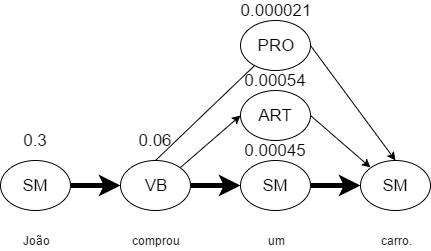
\includegraphics[height=180px]{imagens/markov2.png}
\caption{Caminhos definidos para a classificação pelo Algoritmo de Viterbi}
\label{fig:markov2}
\end{figure}


% Uma maneira de diferenciarmos os dois métodos é através do problema de
% ambiguidade. Por exemplo, nas frases:
%
% ``João entrou no carro conversível de óculos novos.''. E ``João entrou no carro
% conversível de farol apagado.''.
%
% Em ambas as frases, após a preposição ``de'' segue um substantivo masculino.
% Porém, cada uma das frases se refere a um substantivo diferente. A
% primeira se refere ao João, visto que não existe sentido em um carro ter óculos.
% Já a segunda se refere ao próprio carro, visto que não existe sentido em João
% ter faróis.
%
% O método simbólico para resolver esse problema faz a criação de novas regras se
% baseadas no conhecimento humano para a solução de qual o significado da frase.
% Já o método estatístico, irá verificar qual a probabilidade de cada significado
% para cada frase através de análises similares decidindo através de metódos
% estatísticos qual o significado correto para cada frase
% \cite{jacksonmoulinier2007}.

\chapter{Métodos estatísticos e simbólicos aplicados na análise de sentimentos}
\label{cap:Classificadores}

Antigamente, para sabermos a opinião de outras pessoas sobre um
determinado produto, tinhamos que perguntar diretamente. Com a
popularização da Internet e também de redes sociais, milhares de pessoas
compartilham para todos as suas opinões sobre produtos, política, serviços e
demais assuntos. Porém, muitas vezes essas opiniões acabam
por ser esquecidas devido a dificuldade de se analisar uma grande quantidade de
textos. De fato, uma das maiores dificuldades reside em como obter a opinião
geral sobre determinado produto em uma seção de comentários com mais de 1000
opiniões diferentes. Dentro dessa contexto, a análise de sentimentos,
considerada uma tarefa do \ac{NLP}, tem como função identificar e quantificar esses sentimentos expressos através de textos.

Outros possíveis métodos de análise de sentimentos através de aprendizado de
máquina são \ac{SVM} e \ac{MaxEnt}, os quais possuem
performance similar ao Naive Bayes \cite{domingos97naivebayes}.


Neste capítulo serão descritos um método estatístico, Naive Bayes e um método
simbólico, \ac{VADER}, aplicados na análise de sentimentos. Outros possíveis
métodos estatísticos para a análise de sentimentos são \ac{SVM} e \ac{MaxEnt},
os quais possuem performance similar ao Naive Bayes \cite{Pang:2002:TUS:1118693.1118704}. O método simbólico
\ac{VADER} foi selecionado pois este, segundo seus criadores, apresenta
performance superior aos métodos já existentes \cite{conf/icwsm/HuttoG14}.

Ambos métodos selecionados serão descritos para o uso da língua Inglesa,
visto que o \textit{Website} analisado (Reddit) possui a maioria de seus
comentários em língua Inglesa. Além disso, não foram encontrados métodos que
façam uso da língua Portuguesa com similar precisão.




%Para o \ac{NLP} e também para o campo de estatísticas, classificadores são
%algorítmos que identificam a qual categoria determinado item pertence. Essa
%classificação é feita a partir de dados já classificados corretamente, ou seja,
%um \textit{training set}.

\section{Naive Bayes}

O Naive Bayes é um método estatístico para a classificação o qual podemos
aplicar para a análise de sentimento. Esse faz o uso do teorema de Bayes e um
\textit{training set} para inferir a classificação de uma frase. Por exemplo,
precisamos determinar se a frase ``This place is great.'' demonstra um
sentimento negativo ou positivo. 

\begin{table}[htb]
\centering
\begin{tabular}{|l|l|}
\hline
Texto  & Categoria \\ \hline
The food was great  & Positiva     \\ \hline
They are horrible!    & Negativa     \\ \hline
I love the food here  & Positiva     \\ \hline
This place is wonderful  & Positiva     \\ \hline
Forgettable experience  & Negativa     \\ \hline
\end{tabular}
\caption{\textit{Training Set}}
\label{tab:trainingsetnb}
\end{table}

A partir do \textit{training set} hipotético (Tabela
\ref{tab:trainingsetnb}) o método irá calcular a probabilidade da frase ``This
place is great'' ser positiva e também de ser negativa sendo que a partir dessas
duas possibilidades, será escolhida a de maior probabilidade.

Para cálcular a probabilidade da frase ``This place is great'' pertencer a cada categoria
é utilizado o teorema de Bayes \cite{manningschutze1999}, através da Equação
\ref{eq:teorema}.

\begin{equation}
\begin{gathered}
P(c|d) = \frac{P(d|c) \times P(c)}{P(d)} \\
\label{eq:teorema}
\end{gathered}
\end{equation}

\begin{equation}
\begin{gathered}
P(Negativa|\textit{This place is great})
=
\frac{P(\textit{This place is great}|Negativa) \times
P(Negativa)}{\textit{This place is great}}
\label{eq:teoreman1}
\end{gathered}
\end{equation}
\begin{equation}
\begin{gathered}
P(Positiva|\textit{This place is great})
=
\frac{P(\textit{This place is great}|Positiva) \times
P(Positiva)}{\textit{This place is great}}
\label{eq:teoremap1}
\end{gathered}
\end{equation}


Onde o termo P(c$\vert$d) é a probabilidade da frase \textbf{d} pertencer a
classe \textbf{c}. Ou seja, a probabilidade de \textit{``This place is great''} ser
  uma frase positiva ou negativa. O Termo P(d$\vert$c) é a probabilidade da
  classe \textbf{c} ser a frase \textbf{d}. Ou seja, dentre todas as frases
  negativas ou positivas, a probabilidade de uma frase ser \textit{``This place
  is great''}. Já P(c) é a probabilidade da classe \textbf{c}. Ou seja, a frequência que
  frases negativas ou positivas aparecem em nosso \textit{training
  set}. E, por fim, P(d) é a probabilidade de \textbf{d}. Ou seja, a frequência que
  a frase \textit{``This place is great''} aparece em nosso \textit{training
  set}. Como ambas as Equações \ref{eq:teoreman1} e \ref{eq:teoremap1} terão
  como divisor P(d), este pode ser simplificado resultando nas equações
  \ref{eq:teoreman} e \ref{eq:teoremap}.
\begin{equation}
\begin{gathered}
P(Negativa|\textit{This place is great})
=
P(\textit{This place is great}|Negativa) \times
P(Negativa)
\label{eq:teoreman}
\end{gathered}
\end{equation}
\begin{equation}
\begin{gathered}
P(Positiva|\textit{This place is great})
=
P(\textit{This place is great}|Positiva) \times
P(Positiva)
\label{eq:teoremap}
\end{gathered}
\end{equation}

Os termos P(Positiva) e P(Negativa) são definidos pela frequência que frases
positivas e negativas aparecem no \textit{training set}, sendo determinados
através das Equações \ref{eq:frasespositivas} e \ref{eq:frasesnegativas}. Neste
caso, \textit{``The food was great''}, \textit{``I love the food here''}, \textit{``This place is
wonderful''} são frases positivas e as demais frases ``\textit{They are horrible!}'' e
``\textit{Forgettable experience}'' são negativas.

\begin{equation}
\begin{gathered}
P(Positiva)
=
\frac{3}{5} = 0,6
\label{eq:frasespositivas}
\end{gathered}
\end{equation}
\begin{equation}
\begin{gathered}
P(Negativa)
=
\frac{2}{5} = 0,4
\label{eq:frasesnegativas}
\end{gathered}
\end{equation}
Uma vez que a frase \textit{``This place is great''} não existe por completo no
\textit{training set}, tem-se que o termo P(d$\vert$c) da Equação
\ref{eq:teoreman} e \ref{eq:teoremap} é igual a zero (0) (impossibilitando o
cálculo de probabilidade para essa frase). Neste caso, se faz o uso do
\textit{Naive Bayes}, o qual passa a considerar as palavras ao invés de frases
completas, isso elimina o problema com frases que não se
encontram no \textit{training sets}. Neste caso, considera-se somente a
fraquência que cada palavra aparece em uma frase positiva e em uma negativa.
Portanto para o \textit{Naive Bayes} o termo $P(\textit{This place is
great}|Positiva)$ visto na Equação \ref{eq:teoremap} é dado pela Equação
\ref{eq:frasespositivas1}.

\begin{equation}
\begin{gathered}
P(\textit{This place is great}|Positiva) = P(\textit{This}|Positiva)
\times P(\textit{place}|Positiva) \\ \times P(\textit{is}|Positiva) \times
P(\textit{great}|Positiva)
\label{eq:frasespositivas1}
\end{gathered}
\end{equation}

A partir da Equação \ref{eq:frasespositivas1} é necessário calcular os
termos P(\textit{This}$\vert$Positiva),
P(\textit{place}$\vert$Positiva), P(\textit{is}$\vert$Positiva), P(\textit{great}$\vert$Positiva).
O termo P(\textit{This}$\vert$Positiva) é calculado pela razão entre a
quantidade de vezes que a palavra \textit{This} foi classificada como positiva em nosso
\textit{training set}, e o total de palavras classificadas como positiva
(Equação \ref{eq:thispositiva}).

\begin{equation}
\begin{gathered}
P(\textit{This}|Positiva) = \frac{1}{13}
\label{eq:thispositiva}
\end{gathered}
\end{equation}


Da mesma forma, a Equação \ref{eq:thispositiva} deve ser aplicada para as demais
palavras da frase \textit{``This place is great''}, obtendo-se os valores
apresentados na Tabela \ref{tab:probabilidadesnb}.

\begin{table}[htb]
\centering
\renewcommand{\arraystretch}{1.5}% Spread rows out...
\begin{tabular}{lll}
\hline

Palavra & Positiva & Negativa \\ \hline
This & \large $\frac{1}{13}$ & \large $\frac{0}{5}$ \\
place & \large $\frac{1}{13}$ & \large $\frac{0}{5}$ \\
is & \large $\frac{1}{13}$ & \large $\frac{0}{5}$ \\
great & \large $\frac{1}{13}$ & \large $\frac{0}{5}$ \\
\end{tabular}
\caption{Tabela de Palavras e Probabilidades.}
\label{tab:probabilidadesnb}
\end{table}

Uma vez que algumas palavras não encontram-se no \textit{training set}
para determinadas situações, elas acabam zerando o resultado final da
multiplicação das probabilidades de cada palavra (Equação
\ref{eq:frasespositivas1}). De modo, a evitar que uma única palavra
invalide uma frase é utilizado \textit{Laplace smoothing} \cite{Manning:2008:IIR:1394399}. Neste, é
somado 1 a cada palavra e ao total de palavras, são somadas as quantidades de
palavras distintas do \textit{training set} (16). Aplicando o
\textit{Laplace smoothing} para a Tabela \ref{tab:probabilidadesnb} é obtida a
Tabela \ref{tab:probabilidadesl}.


\begin{table}[htb]
\centering
\renewcommand{\arraystretch}{1.5}% Spread rows out...
\begin{tabular}{lll}
\hline

Palavra & Positiva & Negativa \\ \hline
This & \large $\frac{1 + 1}{13 + 16}$ & \large $\frac{0 + 1}{5 + 16}$ \\
place & \large $\frac{1 + 1}{13 + 16}$ & \large $\frac{0 + 1}{5 + 16}$ \\
is & \large $\frac{1 + 1}{13 + 16}$ & \large $\frac{0 + 1}{5 + 16}$ \\
great & \large $\frac{1 + 1}{13 + 16}$ & \large $\frac{0 + 1}{5 + 16}$ \\
\end{tabular}
\caption{Tabela de Probabilidades - \textit{Laplace smoothing}.}
\label{tab:probabilidadesl}
\end{table}

Utilizando as probabilidades obtidas na Tabela
\ref{tab:probabilidadesl} na Equação \ref{eq:frasespositivas1} tem-se:

\begin{equation}
\begin{gathered}
P(Positiva|\textit{This place is great}) = \frac{1 + 1}{13 + 16} \times
\frac{1 + 1}{13 + 16} \times \frac{1 + 1}{13 + 16} \times
\frac{1 + 1}{13 + 16} = 0,000023.
\label{eq:ppositivaplace}
\end{gathered}
\end{equation}

Uma vez que o termo P(Positiva $\vert$ \textit{This place is great})
encontra-se definido através da Equação \ref{eq:ppositivaplace}, pode-se
utilizar a Equação \ref{eq:teoreman}, onde o termo P(Positiva) é igual a 0,6
definido através da Equação \ref{eq:frasespositivas}. Neste caso, tem-se que a
probabilidade da frase \textit{``This place is great''} ser classificada como
positiva é dada através da Equação \ref{eq:positiva}.

\begin{equation}
\begin{gathered}
P(Positiva|\textit{This place is great})
=
0,000023 \times
0,6 = 0,0000138.
\label{eq:positiva}
\end{gathered}
\end{equation}

Efetuando o mesmo processo para a probabilidade da frase ser negativa, tem-se:
\begin{equation}
\begin{gathered}
P(Negativa|\textit{This place is great})
=
0,0000049 \times
0,4 = 0,00000196.
\label{eq:negativa}
\end{gathered}
\end{equation}

Portanto, tem-se que a frase ``This place is great'' é positiva, uma vez que a
probabilidade de ser positiva (0,0000138) é maior que a probabilidade dessa
frase ser negativa (0,00000196).

\section{\textit{VADER}}

O \ac{VADER} é um dicionário e classificador de sentimentos que se baseia em
regras, portanto, um método de classificação simbólico. Esse foi desenvolvido
especificadamente para funcionar em redes sociais onde-se tem um contexto
vago, pouca quantidade de texto, gírias e emoticons \cite{conf/icwsm/HuttoG14}.

A classificação do sentimento é feita através da separação da frase em palavras
e para cada palavra da frase é atribuída uma pontuação de intensidade em uma
escala de -4 até +4. Como por exemplo, a palavra \textit{great} tem a
intensidade de 3.1 e \textit{horrible} -2.5. Essa pontuação é obtida através de
um dicionário que é construído utilizando o método de \textit{``wisdom of the
crowd''} onde um grupo de pessoas atribuiu os valores de intensidade para cada palavra. Por
exemplo, a frase \textit{``This place is great''} seria classificada com:


\begin{table}[htb]
\centering
\begin{tabular}{l|l|l|l|l|l|l}
Palavra         & \textit{This}        & \textit{place} & \textit{is}      &
\textit{great}
\\
%Correta: & Substantivo & Verbo  & Artigo & Substantivo & Preposição &
% Substantivo \\
Intensidade:   &  &   &  & 3,1
\end{tabular}
\label{my-label}
\end{table}

As palavras \textit{``This''}, \textit{``place''} e \textit{``is''} são
desconsideradas uma vez que não existem no dicionário e não expressam
sentimentos. Após, ele faz uso do seguinte conjunto de regras para inferir a
intensidade do sentimento:
\begin{itemize}
\item A primeira regra consistem em verificar quando uma palavra com pontuação
atribuída (uma palavra que expressa sentimentos) é escrita em letras
maiúsculas.
  Neste caso, é aumentada a magnitude da intensidade do sentimento sem modificar
  a orientação semântica. Para isso, é somado 0,733 a intensidade do
  sentimento caso este tenha intensidade positiva ou subtraído
  0,733 caso este tenha intensidade negativa.
  \begin{table}[htb]
	\centering
	\begin{tabular}{l|l|l|l|l|l|l}
	Palavra         & \textit{This}        & \textit{place} & \textit{is}      &
	\textit{GREAT}
	\\
	%Correta: & Substantivo & Verbo  & Artigo & Substantivo & Preposição &
	% Substantivo \\
	Intensidade:   &  &   &  & 3,1 \textrightarrow 3,833
	\end{tabular}
	\label{my-label}
   \end{table}

\item A segunda regra verifica se alguma das três palavras anteriores é um advérbio intensificador. Neste caso, estes impactam a
intensidade do sentimento aumentando ou diminuindo 0,293 conforme o advérbio. 
  \begin{table}[htb]
	\centering
	\begin{tabular}{l|l|l|l|l|l|l}
	Palavra         & \textit{This}        & \textit{place} & \textit{is}      &
	\textit{incredibly} & \textit{great}
	\\
	%Correta: & Substantivo & Verbo  & Artigo & Substantivo & Preposição &
	% Substantivo \\
	Intensidade:   &  &   &  & Advérbio & 3,1 \textrightarrow 3,393 
	
	\end{tabular}
	\label{my-label}
   \end{table}
   
   
  \begin{table}[htb]
	\centering
	\begin{tabular}{l|l|l|l|l|l|l}
	Palavra         & \textit{This}        & \textit{place} & \textit{is}      &
	\textit{somewhat} & \textit{great}
	\\
	%Correta: & Substantivo & Verbo  & Artigo & Substantivo & Preposição &
	% Substantivo \\
	Intensidade:   &  &   &  & Advérbio & 3,1 \textrightarrow 2,807
	\end{tabular}
	\label{my-label}
   \end{table}
   

\item A terceira regra verifica se a frase contém a palavra \textit{``but''}.
Caso encontrada, essa palavra indica uma troca do sentimento da frase, uma vez
que o texto seguinte a palavra \textit{``but''} expressa um sentimento mais
dominante. Neste caso, o método multiplica a intensidade dos sentimentos
expressos até a palavra \textit{``but''} por 0,5 e os sentimentos expressos após a palavra \textit{``but''} por 1,5.

   
   \begin{table}[!htbp]
	\centering
	\begin{tabular}{l|l|l|l|l|l|l|l|l}
	Palavra         & \textit{Great} & \textit{place}      & \textbf{\textit{but}}
	& \textit{today} & \textit{the}      &
	\textit{food} & \textit{was}      & \textit{horrible}
	\\
	%Correta: & Substantivo & Verbo  & Artigo & Substantivo & Preposição &
	% Substantivo \\
	Intensidade: & 3,1 \textrightarrow 1,55  &   &  &  & & & &  -2,5
	\textrightarrow -3,75
	\end{tabular}
	\label{my-label5}
   \end{table}

\item A quarta regra verifica se a frase possui pontos de exclamação (!). Este
tipo de pontuação aumenta a magnitude da intensidade sem modificar a
orientação semântica. 0,292 a cada ponto de exclamação considerando um
máximo de 4 pontos de exclamação.

 \begin{table}[!htbp]
	\centering
	\begin{tabular}{l|l|l|l|l|l|l}
	Palavra         & \textit{This}        & \textit{place} & \textit{is}      &
	\textit{great!}
	\\
	%Correta: & Substantivo & Verbo  & Artigo & Substantivo & Preposição &
	% Substantivo \\
	Intensidade:   &  &   &  & 3,1 \textrightarrow 3,392
	\end{tabular}
	\label{my-label}
   \end{table}
   

\item Por fim, a quinta regra examina as três palavras anteriores,
procurando a existência de uma negação que inverte a polaridade de um texto.
Quando é encontrada uma negação na frase, a intensidade de cada palavra de
sentimento é multiplicada por -0,74.

 \begin{table}[!htbp]
	\centering
	\begin{tabular}{l|l|l|l|l|l|l}
	Palavra         & \textit{This}        & \textit{place} & \textit{wasn't}     
	&
	\textit{great}
	\\
	%Correta: & Substantivo & Verbo  & Artigo & Substantivo & Preposição &
	% Substantivo \\
	Intensidade:   &  &   & Negação & 3,1 \textrightarrow 2,294
	\end{tabular}
	\label{my-label}
   \end{table}


\end{itemize}

Após esse cálculo de pontuação de intensidade, é feita a normalização dessa
pontuação através da Equação \ref{eq:vader}.

\begin{equation}
\begin{gathered}
\text{Pontuação Normalizada}
=
\frac{\text{Pontuação}}{\sqrt{\text{Pontuação}^2 + 15}}
\label{eq:vader}
\end{gathered}
\end{equation}


\begin{equation}
\begin{gathered}
\text{Pontuação Normalizada}
=
\frac{\text{3,1}}{\sqrt{\text{3,1}^2 + 15}} = 0,6249
\label{eq:vaderscore}
\end{gathered}
\end{equation}

Neste caos para a frase \textit{``This place is great''} (aonde somente a
palavra \textit{great} possui pontuação e essa tem o valor de 3,1) será
atribuida pontuação final de 0,6249.  Caso essa
pontuação fosse menor que -1 ou maior que 1, essa seria limitada aos valores de
-1 ou 1 respectivamente. Para o \ac{VADER}, são consideradas frases negativas aquelas
com pontuação de -1 até -0,5, frases neutras aquelas com pontuação de -0,5 até
0,5 e frases positivas aquelas com pontuação 0,5 até 1. Portanto a frase
\textit{``This place is great''} com pontuação 0,6249 seria classificada como
positiva.
